\documentclass[10pt,a4paper]{article}
\usepackage[margin=1.25in]{geometry}
\usepackage{fancyhdr} % fancy header
\pagestyle{fancy} % so fancy
\usepackage[round]{natbib} % bibliography
\usepackage{graphicx} % for importing graphics / figures
\usepackage{booktabs} % publication-worthy tables
\usepackage{adjustbox} % makes tables fit nicely on the page


\lhead{Josh MEYER}
\rhead{Dissertation Prospectus}
\cfoot{} %% make empty to get rid of the page number %% \cfoot{Page \thepage}
\renewcommand{\footrulewidth}{0.4pt} %% this puts a fancy line at the footer


\begin{document}


\section{What I'm doing \& Why it's Extremely Cool}

I'm creating Neural Nets which better classify data from unseen conditions, without any explicit adaptation of model parameters or data transformations.

My approach is extremely cool because it doesn't require tons of data, it is not specific to some dataset, and it can be used to build any Neural Net (not just for speech recognition).


\section{Overview of Speech Recognition}

This section contains an overview of the training and testing procedures for standard automatic speech recognition (ASR) pipelines. The overview will provide the reader with a technical grounding in ASR, so that the rest of the dissertation will have some point of reference. 


\begin{itemize}

\item \textbf{Gaussians + HMMs}
  
\item \textbf{Neural Nets + HMMs}
  
\item \textbf{end-to-end Neural Nets}

\end{itemize}


\section{Background Literature}

Here I will cover the literature relevant to working with small (or completely new) datasets. There are two main approaches, (1) adapt a model from one training dataset to a new, smaller dataset; (2) create a model that is robust enough to handle data from multiple domains. 

\begin{itemize}

\item \textbf{Model Adaptation: (e.g. Speaker; Language)}

      %% 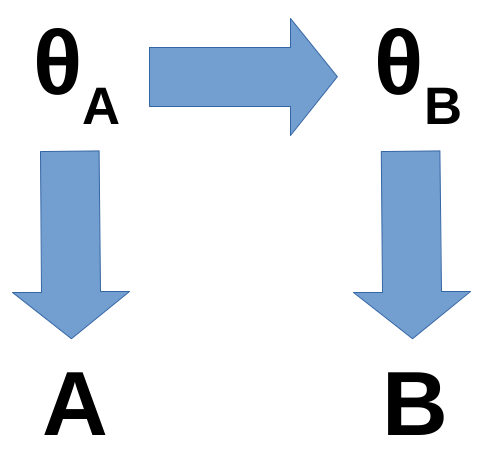
\includegraphics[width=.2\textwidth,keepaspectratio]{figs/transfer.png}
    
  
\item \textbf{Model Robustness: (e.g. Noise; Channel)}

    %% 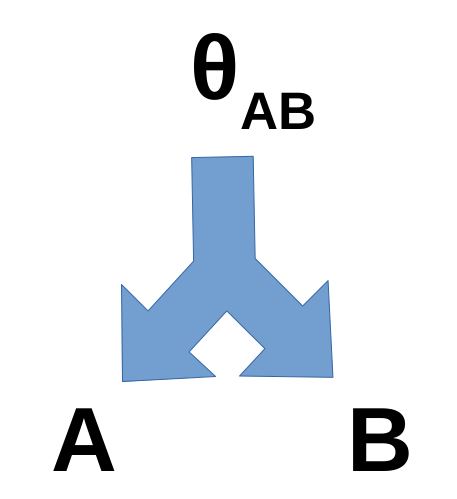
\includegraphics[width=.2\textwidth,keepaspectratio]{figs/robustness.png}
  
\end{itemize}




\section{Experiments}

This section contains the main contributions of the dissertation research.

The aim of the dissertation is to investigate training methods for acoustic modeling to be used in the Neural Net + HMM ASR pipeline.

\subsection{Data}
I aim to produce acoustic models which perform better (i.e. lower Word Error Rates) on datasets which are not similar the original training dataset.

The differences between the training and testing data will be (1) the recording noise conditions, (2) who the speaker is, or (3) what language the speaker is using.


\begin{table}[htbp]
  \centering
  \begin{adjustbox}{width=.5\textwidth}
    \begin{tabular}{lll}
      \toprule
      & \textbf{Train} & \textbf{Test}\\
      \midrule
      \textbf{Noise} & TIDIGITS & Aurora 5 \\
      \textbf{Speaker} & LibriSpeech-A & LibriSpeech-B \\
      \textbf{Language} & LibriSpeech & Kyrgyz Audiobook \\
      \bottomrule
    \end{tabular}
    \label{table:data}
  \end{adjustbox}
  
  \caption{Speech Corpora}
  
\end{table}



In particular, I will investigate methods of neural net training with Multi-Task Learning. Mutli-Task Learning has a long history of producting robust classifiers by learning representations of the data which are useful in performing all tasks (Caruna 1997).

Typically, these tasks are assumed to exist and are useful in some other application (e.g. POS tagging and dependency parsing combined as two tasks). However, a less common approach is to create completely new tasks for the sake of Multi-Task Learning.

This dissertation investigates the creation of new tasks, either using linguist-expert knowledge, ASR Engineer-expert knowledge, or general machine learning concepts. The latter two genres of tasks can only be used in buidling acoustic models, but the final approach leveraging machine learning concepts could be applied to any classification problem on any dataset. For example, you can train an image classifier with the latter methods, but not with the former.


\begin{itemize}

\item \textbf{Multi-task Learning}

Ways to construct the mutliple tasks using:
  
  \begin{itemize}
    
  \item \textbf{Linguistic Knowledge}
    
  \begin{itemize}  
  \item \textbf{Tasks == classification based on phonetic categories  \\ (e.g. vowels vs. consonants)}
  \end{itemize}
  
  \item \textbf{Traditional Speech Recognition Pipeline}
  \begin{itemize}  
  \item \textbf{Tasks == classification based on phoneme classification tree \\ (e.g. monophones vs. triphones)}
  \end{itemize}
    
  \item \textbf{General Machine Learning}
  \begin{itemize}  
  \item \textbf{Tasks == classification based on new labels \\ (e.g. from k-means; random forests) / data sub-sets (e.g. bootstrap resampling)}
  \end{itemize}
  \end{itemize}
  
\end{itemize}


\end{document}



 
